\documentclass{article}
\usepackage{amsmath}
\usepackage{amssymb}
\usepackage{amsfonts}
\usepackage{paracol}
\usepackage[inline]{enumitem}
\usepackage{geometry}
\usepackage{tikz}
\usetikzlibrary{angles,quotes}
\geometry{a4paper, left=15mm, top=15mm, right=15mm, bottom=15mm}
\title{Chapter 18

  Advanced Trigonometry}
\date{}
\begin{document}
\maketitle
\section{Radian and Degree Measures}
% example 1
\subsection{Convert them into degree measure}
\paragraph{Example 1:}
\begin{enumerate}
        \begin{paracol}{3}
          \item[a.] $\frac{\pi}{6}$
          \item[d.] $\frac{7\pi}{6}$
          \item[g.] $\frac{7\pi}{18}$
          \switchcolumn
          \item[b.] $\frac{4\pi}{5}$
          \item[e.] $\frac{8\pi}{3}$
          \switchcolumn
          \item[c.] $\frac{11\pi}{6}$
          \item[f.] $\frac{7\pi}{4}$
          \switchcolumn
        \end{paracol}
\end{enumerate}
{\footnotesize Since $\pi=180^{0}$, $1 radian = \frac{180^{0}}{\pi}$ OR $1^{0} = \frac{\pi}{180^{0}}$}

\paragraph{Solutions:}
\begin{enumerate}
        \begin{paracol}{3}
          \item[a.] $\frac{\pi}{6} \times \frac{180^{0}}{\pi} = 30^{0}$
          \item[d.] $\frac{7\pi}{6} \times \frac{180^{0}}{\pi} = 210^{0}$
          \item[g.] $\frac{7\pi}{18} \times \frac{180^{0}}{\pi} = 70^{0}$
          \switchcolumn
          \item[b.] $\frac{4\pi}{5} \times \frac{180^{0}}{\pi} = 144^{0}$
          \item[e.] $\frac{8\pi}{3} \times \frac{180^{0}}{\pi} = 480^{0}$
          \switchcolumn
          \item[c.] $\frac{11\pi}{6} \times \frac{180^{0}}{\pi} = 330^{0}$
          \item[f.] $\frac{7\pi}{4} \times \frac{180^{0}}{\pi} = 315^{0}$
          \switchcolumn
        \end{paracol}
\end{enumerate}

% example 2
\subsection{Convert them to radian measure}
\paragraph{Example 2:}
\begin{enumerate}
        \begin{paracol}{3}
          \item[a.] $\theta=5^{'}$
          \item[d.] $330^{0}$
          \item[g.] $520^{0}$
          \switchcolumn
          \item[b.] $-120^{0}$
          \item[e.] $480^{0}$
          \item[h.] $240^{0}$
          \switchcolumn
          \item[c.] $210^{0}$
          \item[f.] $-47^{0}30^{'}$
          \item[i.] $-7^{0}30^{'}$
          \switchcolumn
        \end{paracol}
\end{enumerate}

\paragraph{Solutions :}
\begin{enumerate}
        \begin{paracol}{3}
          \item[a.] $\theta=5^{'}=\frac{5^{0}}{60} \times \frac{\pi}{180^{0}} = \frac{\pi}{12 \times 180} radians$
          \item[d.] $330^{0} = 330^{0} \times \frac{\pi}{180^{0}} = \left(\frac{11\pi}{6}\right)^{c}$
          \item[g.] $520^{0} = -520 \times \frac{\pi}{180^{0}} = \frac{26\pi}{9} $
          \switchcolumn
          \item[b.] $-120^{0} \times \frac{\pi}{180^{0}} = \left(\frac{-2 \pi}{3}\right)^{c}$
          \item[e.] $480^{0} = 480^{0} \times \frac{\pi}{180^{0}} = \frac{8\pi}{3}$
          \item[h.] $240^{0} = 240^{0} \times \frac{\pi}{180^{0}} = \frac{4\pi}{3}$
          \switchcolumn
          \item[c.] $210^{0} = 210^{0} \times \frac{\pi}{180^{0}} = \frac{7\pi}{6}$
          \item[f.] $-47^{0}30^{'} = -47\frac{1}{2}^{0} \\
          = \left(\frac{-95}{2}^{0}\right) \times \frac{\pi}{180^{0}} \\
          = \frac{-19\pi}{72} $
          \item[i.] $-7^{0}30^{'} = 7\frac{1}{2}^{0} \\
          = 7\frac{1}{2}^{0} \times \left(\frac{\pi}{180}\right)^{c} \\
          = \frac{15}{2} \times \left(\frac{\pi}{180}\right)^{c} \\
          = \left(\frac{\pi}{24}\right)^{c}$
          \switchcolumn
        \end{paracol}
\end{enumerate}

% example 3
\subsection{Sine, Cosine and Tangents}
\paragraph{Example 3: Without using calculator, solve the following questions}
\begin{enumerate}
  \item[a.] If $\sin(18^{0})= 0.309$, give another angle whose $\sin$ is $0.309$.
        
        {\small Solution: since}
        \[
        \begin{aligned}
          \sin(180^0-\theta) = \sin(\theta)
          &\therefore \sin(180^{0}-18^{0}) = \sin(162^{0}) \\
          &\therefore \theta = 162^{0}
        \end{aligned}
        \]

  \item[b.] If $\cos(70^{0})= 0.342$, give another angle whose $\cos$ is $0.342$.

        {\small Solution: since}
        \[
        \begin{aligned}
          \cos\theta = \cos(2\pi - \theta)
          &\therefore \cos(360-70^{0}) = \cos(290^{0}) \\
          &\therefore \theta = 290^{0}
        \end{aligned}
        \]

  \item[c.] If $\cos(300^{0})= \frac{1}{2}$, give another angle whose $\cos$ is $\frac{1}{2}$.

        {\small Solution: since}
        \[
        \begin{aligned}
          \cos(300^{0}) &= \cos(360-60^{0}) = \cos(60^{0}) \\
                       &\therefore \theta = 60^{0}
        \end{aligned}
        \]

  \item[d.] If $\cos(120^{0})= \frac{-1}{2}$, give another angle whose $\cos$ is $-0.5$.

        {\small Solution: since}
        \[
        \begin{aligned}
          \cos\theta = \cos(360-\theta)
          &\therefore \cos(120^{0}) = \cos(360^{0} - 120^{0}) = \cos(240^{0}) \\
          &\therefore \theta = 240^{0}
        \end{aligned}
        \]

  \item[e.] (Use Calculator) If $\sin(x)= 0.848$, find two values for $x$ between $0^{0}$ and $360^{0}$.

        \[
        \begin{aligned}
          x = 58^{0}, 122^{0}
        \end{aligned}
        \]
\end{enumerate}

\paragraph{Example 4:}
If $\tan\theta = \frac{1}{\sqrt{3}}$, find the other values of a) $\sin\theta$ b) $\cos\theta$

{\small Solutions:}
\begin{enumerate}
        \item[a.]
        \[
        \begin{aligned}
          \sec^{2}\theta = \tan^{2}\theta + 1 = \frac{1}{3}+1 = \frac{4}{3} \\
          \therefore \sec\theta = \pm\frac{2}{\sqrt{3}} \Rightarrow \cos\theta = \pm \frac{\sqrt{3}}{2}
        \end{aligned}
        \]

        \item[b.]
        \[
        \begin{aligned}
          \sin\theta^{2}\theta = 1 - \cos^{2}\theta = 1 - \frac{3}{4} = \frac{1}{4} \\
          \therefore \sin\theta = \pm\frac{1}{2}
        \end{aligned}
        \]
\end{enumerate}

\paragraph{Example 5:}
If $\sin\theta = \frac{1}{\sqrt{2}}$, find the values of a) $\cos\theta$ b) $\tan\theta$

{\small Solutions:}
\begin{enumerate}
        \item[a.]
        \[
        \begin{aligned}
          \cos^{2}\theta = 1 - \sin^{2}\theta = 1 - \frac{1}{2} = \frac{1}{2} \\
          \cos\theta = \pm\frac{1}{\sqrt{2}} \\
        \end{aligned}
        \]

        \item[b.]
        \[
        \begin{aligned}
          \tan\theta = \frac{\sin\theta}{\cos\theta} = \frac{1/\sqrt{2}}{\pm\frac{1}{\sqrt{2}}} = \pm 1
        \end{aligned}
        \]
\end{enumerate}

Alternatively, we can find these values by drawing a right angle triangle.

\begin{center}
  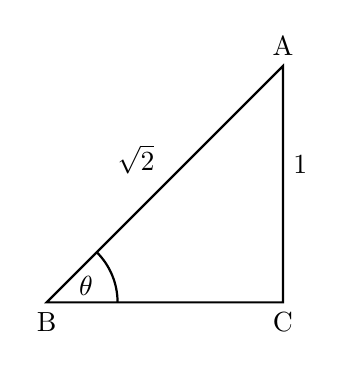
\begin{tikzpicture}[thick]
    % Draw the triangle
    \coordinate (A) at (3,3);
    \coordinate (B) at (0,0);
    \coordinate (C) at (3,0);

    \draw (A) -- (B) -- (C) -- cycle;

    % Add labels
    \node[above] at (A) {A};
    \node[below] at (B) {B};
    \node[below] at (C) {C};
    \draw (1.5, 1.5) node[above left]{$\sqrt{2}$};
    \draw (3.0, 1.5) node[above right]{$1$};

    % Draw angles with markers
    \pic [draw, angle radius=9mm, "$\theta$"] {angle = C--B--A};
  \end{tikzpicture}
\end{center}

{\small Solution:}
\[ \sin\theta = \frac{1}{\sqrt{2}} \]
Applying Pythagoras theorem
\[
  \begin{aligned}
    BC^{2} = AB^{2} - AC^{2} = 2 - 1 = 1 \\
    BC = 1
  \end{aligned}
\]
$\therefore$

\[
  \begin{aligned}
    \cos\theta = \frac{BC}{AB} = \frac{1}{\sqrt{2}} \\
    \tan\theta = \frac{AC}{BC} = \frac{1}{1} = 1
  \end{aligned}
\]

\subsection{Verifying Trigonometric Identities}
\paragraph{Example 6: Verify each of the following by putting values}

\begin{enumerate}
  \item[a.] $\sin 60^{0} \cos 30^{0} - \cos 60^{0} \sin 30^{0} = \sin 30^{0} \Rightarrow \frac{\sqrt{3}}{2} \times \frac{\sqrt{3}}{2} - \frac{1}{2} \times \frac{1}{2} = \frac{3-1}{4}=\frac{1}{2}$
  \item[b.] $\cos 60^{0} \cos 30^{0} + \sin 60^{0} \sin 30^{0} = \cos 30^{0} \Rightarrow \frac{1}{2} \times \frac{\sqrt{3}}{2} + \frac{\sqrt{3}}{2} \times \frac{1}{2} = \frac{\sqrt{3}}{2}$
  \item[c.] $2 \sin 30^{0} \cos 30^{0} = \sin 60^{0} \Rightarrow 2 \times \frac{1}{2} \times \frac{\sqrt{3}}{2} = \frac{\sqrt{3}}{2}$
  \item[d.] $\cos 60^{0} = 2 \cos^{2} 30^{0} - 1 \Rightarrow 2 \times \left(\frac{\sqrt{3}}{2}\right)^{2} - 1 = 2 \times \frac{3}{4} - 1 = \frac{1}{2}$
  \item[e.] $\cos 60^{0} = 1 - 2 \sin^{2} 30^{0} \Rightarrow 1 - 2 \times \left(\frac{1}{2}\right)^{2} = 1 - \frac{1}{2} = \frac{1}{2}$
\end{enumerate}

\paragraph{Example 7:}
Using the formula $\cos A = \sqrt\frac{1+\cos2A}{2}$ and $\sin A = \sqrt\frac{1-\cos2A}{2}$
find the value of $\cos30^{0}$ and $\sin30^{0}$.

{\small Solution:}

\[
  \begin{aligned}
    \cos30^{0} = \sqrt\frac{1+\cos60^{0}}{2} =  \sqrt\frac{1+\frac{1}{2}}{2} = \sqrt\frac{3}{4} = \frac{\sqrt{3}}{2} \\
    \sin30^{0} = \sqrt\frac{1-\cos60^{0}}{2} =  \sqrt\frac{1-\frac{1}{2}}{2} = \sqrt\frac{1}{4} = \frac{1}{2} \\
  \end{aligned}
\]

\paragraph{Example 8:}
If $A = 60^{0}, B = 30^{0}$, verify

\begin{enumerate}
  \item[a.] $\sin(A-B) = \sin(A) \cos(B) - \cos(A) \sin(B)$
  \item[b.] $\cos(A-B) = \cos(A) \cos(B) - \sin(A) \sin(B)$
  \item[c.] $\tan(2A) = \frac{2\tan(A)}{1-\tan^{2}(A)}$
  \item[a.] $\sin(60^{0}-30^{0}) = \sin60^{0}\cos30^{0} - \cos60^{0}\sin30^{0}$ \\
        $ \frac{1}{2} = \frac{\sqrt{3}}{2} \times \frac{\sqrt{3}}{2} - \frac{1}{2} \times \frac{1}{2} = \frac{3}{4} - \frac{1}{4} = \frac{1}{2} $
  \item[b.] $\cos(60^{0}-30^{0}) = \cos60^{0}\cos30^{0} + \sin60^{0}\sin30^{0}$ \\
        $ \frac{\sqrt{3}}{2} = \frac{1}{2} \times \frac{\sqrt{3}}{2} + \frac{\sqrt{3}}{2} \times \frac{1}{2} = 2 \times \frac{\sqrt{3}}{4} = \frac{\sqrt{3}}{2}$
  \item[c.] $\tan(2A) = \frac{2\tan(A)}{1-\tan^{2}(A)}$ \\
        $ \tan 60^{0} = \frac{2\tan30^{0}}{1-\tan^{2}30^{0}} = \frac{2\frac{1}{\sqrt{3}}}{1-\frac{1}{3}} = \frac{2\frac{1}{\sqrt{3}}}{\frac{2}{3}} = \sqrt{3} \frac{\sqrt{3}}{\sqrt{3}} = \sqrt{3}$ \\
        $\therefore \sqrt{3} = \sqrt{3}$
\end{enumerate}

\paragraph{Example 9:}
If $A = 30^{0}$, verify $\cos3A = 4\cos^{3}A - 3 \cos(A) $ and $\sin3A = 3\sin(A) - 4\sin^{3}A$

{\small Solution:}

\[
  \begin{aligned}
    \cos(3 \times 30^{0}) &= 4\cos^{3}30^{0} - 3\cos30^{0} \\
                         &= 4\left(\frac{\sqrt{3}}{2}\right)^{2} - 3\frac{\sqrt{3}}{2} \\
                         & 0 = 4 \times \frac{3\sqrt{3}}{4\times2} - \frac{3\sqrt{3}}{2} = 0 \\
                         &\Rightarrow 0 = 0 \\
    \\
    \sin(3 \times 30^{0}) &= 3\sin30^{0} - 4\sin^{3}30^{0} \\
                         & 1 = 3 \times \frac{1}{2} - 4 \times \frac{1}{8} \\
                         & = \frac{3}{2} - \frac{1}{2} \\
                         & = 1 \\
                         &\Rightarrow 1 = 1
  \end{aligned}
\]

\paragraph{Example 10:}
If $\tan(A+B) = \sqrt{3}, \tan(A-B)=\frac{1}{\sqrt{3}}$, find A and B.

{\small Solution:}

$\tan(A+B) = \sqrt{3}, \tan(A-B) = \sqrt{3} \Rightarrow A + B = 60, A - B = 30$

On solving, $A = 45^{0}, B = 15^{0}$

\paragraph{Example 11:}
Using formulae $\sin\theta = \cos(90-\theta)$ and $\cos\theta = \sin(90-\theta)$, evaluate the following.

\begin{enumerate}
        \begin{paracol}{2}
          \item[i.] $\frac{\cos53^{0}}{\sin37^{0}} \times \frac{\sin60^{0}}{\cos30^{0}}$
          \item[iii.] $\tan60^{0} - \cot30^{0}$
          \switchcolumn
          \item[ii.] $\cos^{2}13^{0} - \sin^{2}77^{0}$
          \item[iv.] Prove $\cos^{2}65^{0} + \cos^{2}25^{0} = \sin^{2}65^{0} + \sin^{2}25^{0}$
          \switchcolumn
        \end{paracol}
\end{enumerate}

{\small Solutions:}

\begin{enumerate}
        \begin{paracol}{2}

          \item[i. ] $ \frac{\cos53^{0}}{\sin37^{0}} \times \frac{\sin60^{0}}{\cos30^{0}} \\
          = \frac{\sin(90-53^{0})}{\sin37^{0}} \times \frac{\frac{\sqrt{3}}{2}}{\frac{\sqrt{3}}{2}} \\
          = \frac{\sin37^{0}}{\sin37^{0}} \\
          = 1 $

          \item[iii. ] $\tan60^0 - \cot30^0 \\
          = \tan60^0 - \cot(90^0-30^{0}) \\
          = \tan60^0 - \tan60^0 \\
          = 0$

          \switchcolumn

          \item[ii. ] $\cos^{2}13^0 - \sin^{2}77^0 \\
          = \sin^2(90^0-13^0) - \sin^{2}77^0 \\
          = \sin^{2}77^0 - \sin^{2}77^0 \\
          = 0$

          \item[iv. ]
          \[
            \begin{aligned}
              \cos^{2}65^{0} + \cos^{2}25^{0} &= \cos^{2}65^{0} + \cos^{2}(90^{0}-65^{0}) \\
                                              &= \cos^{2}65^{0} + \sin^{2}65^{0} \\
                                              &= 1 \\
              \sin^{2}65^{0} + \sin^{2}25^{0} &= \sin^{2}65^{0} + \sin^{2}(90^{0}-65^{0}) \\
                                              &= \sin^{2}65^{0} + \cos^{2}65^{0} \\
                                              &= 1
            \end{aligned}
          \]
        \end{paracol}
\end{enumerate}

\paragraph{Example 12:}

\begin{enumerate}
        \item[a.] $\sin(x) = \frac{1}{2}, 0 < x \leq 3\pi$, find all the values of $x$.

        {\scriptsize \textbf{Solution:}}
        $x = \frac{\pi}{6}, \frac{5\pi}{6}, \frac{13\pi}{6}, \frac{17\pi}{6}$

        {\scriptsize \textbf{Note:}}
        $\sin\theta = \sin(180-\theta)$ and $\sin(x) = \sin\theta \\
        x = \theta, \pi - \theta, \theta + 2\pi, 3\pi - \theta
        $

        \item[b.] $\cos(x) = \frac{1}{2}, -2\pi \leq x \leq 2\pi$, find all the values of $x$.

        {\scriptsize \textbf{Solution:}}
        $x = \frac{\pi}{6}, \frac{5\pi}{3}, \frac{-\pi}{6}, \frac{-5\pi}{3}$

        {\scriptsize \textbf{Note:}}
        $x =  \left. \begin{array}{c} \theta \\ \pi-\theta \end{array} \right\} + 2K\pi \\
        $where $K = -2, -1, 0, 1, 2$

        \item[c.] $\tan(x) = \sqrt{3}, 0 \leq x \leq 3\pi$, find all the values of $x$.

        {\scriptsize \textbf{Solution:}}
        $x = \frac{\pi}{3}, \frac{4\pi}{3}, \frac{7\pi}{3}$

        {\scriptsize \textbf{Note:}}
        $\left[ \begin{array}{cc} \tan(x) = \tan\theta \\ x = \theta, \theta + K\pi \end{array} \right] \\
        $where $K = -2, -1, 0, 1, 2$

\end{enumerate}

\end{document}
